\documentclass[11pt,a4paper]{article}
\usepackage[T1]{fontenc}
\usepackage[utf8]{inputenc}
\usepackage{lmodern}
\usepackage[margin=2.5cm]{geometry}
\usepackage{microtype}
\usepackage{amsmath,amssymb}
\usepackage{graphicx}
\usepackage{booktabs,tabularx,array}
\usepackage[dvipsnames]{xcolor}
\usepackage{enumitem}
\usepackage[font=small,labelfont=bf]{caption}
\usepackage[authoryear,round]{natbib}
\usepackage{newunicodechar}
\usepackage[colorlinks,linkcolor=MidnightBlue,citecolor=MidnightBlue,urlcolor=MidnightBlue]{hyperref}

\newunicodechar{→}{\ensuremath{\rightarrow}}
\newunicodechar{≥}{\ensuremath{\geq}}
\newunicodechar{≈}{\ensuremath{\approx}}
\newunicodechar{±}{\ensuremath{\pm}}
\newunicodechar{−}{\ensuremath{-}}
\newunicodechar{×}{\ensuremath{\times}}
\newunicodechar{·}{\ensuremath{\cdot}}
\newunicodechar{ρ}{\ensuremath{\rho}}
\newunicodechar{κ}{\ensuremath{\kappa}}
\newunicodechar{∈}{\ensuremath{\in}}

\setlength{\parskip}{0.4em}
\setlength{\parindent}{0pt}
\renewcommand{\floatpagefraction}{0.75}

\title{Typing the rare neurons of an unlabeled connectome by their wiring: a transferred GNN selects the candidates, graph matching types them}
\author{Maximilian Vogt\thanks{Code, protocols and the command for every number:
\url{https://github.com/Paradoxsmile/flybrain}.}}
\date{Draft v0.4, October 2026}

\begin{document}
\maketitle
\begin{abstract}

New connectome reconstructions are typed by matching their neurons to an annotated reference. Most cell types are rare, with two to four neurons per brain, and connectivity-based typing needs labeled partners in the target. We type rare neurons without any target label in two stages. A graph neural network that sees only anonymous wiring, transferred from the reference, selects the candidate neurons, and graph matching against the reference's rare-type neurons assigns their types. We tested the method under protocols committed before any run on held-out data. On the sparse BANC brain it raised rare-type accuracy from 22 to 41~\%; from the male nerve cord MANC to the nerve cords of BANC and of the male CNS, from 40 to 61~\% and from 72 to 82~\%. References built from morphology or from curated typing gave the same gains. Wiring complements morphology: on BANC's brain, automatic morphology matches (NBLAST) alone type 67~\% of the rare-type neurons, and taking the matched type wherever graph matching assigns a neuron raises this to 73~\% (exploratory). The approach needs the target's full wiring: a partial volume, the hemibrain, cannot be typed this way.

\end{abstract}

\section{Introduction}\label{sec:intro}

Electron-microscopy connectomes of the adult \emph{Drosophila} central nervous system now exist for several individuals: the female FAFB/FlyWire brain (\citealp{dorkenwald2024}; \citealp{schlegel2024}), the hemibrain (\citealp{scheffer2020}), the male ventral nerve cord MANC (\citealp{takemura2024}; \citealp{marin2024}), the male CNS (MCNS; \citealp{berg2026}) and the female brain and nerve cord BANC (\citealp{bates2026}). Their value rests on cell-type annotations. New reconstructions are typed by matching their neurons to an annotated reference, by morphology and by connectivity (\citealp{schlegel2024}; \citealp{bates2026}). Most of the types are small: of FlyWire's 8,772 cell types, about three quarters have two to four neurons. Connectivity-based typing compares each neuron's synaptic partners by type, as in the definition of optic-lobe types (\citealp{matsliah2024}) and in NTAC (\citealp{schwartzman2026}), and therefore needs labeled partners in the target.

We study these rare types in a target in which no neuron is labeled, using only the anonymous wiring diagram, the directed graph of neurons and synapse counts. A classifier trained on the reference has seen one or two examples of each rare type. But these types were defined by matching neurons across hemispheres and brains, and pairing neurons is what graph matching does without labels (\citealp{pedigo2023}). Graph matching needs to know which target neurons to pair, though. We therefore let a graph neural network (GNN), trained on the reference and transferred to the target without labels, decide which neurons to match, and graph matching decide their types. Our contributions:

\begin{enumerate}[leftmargin=*,itemsep=2pt]

\item \textbf{Label-free typing of rare types by a GNN and graph matching} (Figure~\ref{fig:1}). Within FlyWire, graph matching types the right-hemisphere neurons of 2–4-neuron types at 92~\%, against 76~\% for the GNN. Between FlyWire and the male CNS, the label-free combination raises these types from 54 to 75~\% (Section~\ref{sec:res-dev}).

\item \textbf{Pre-registered tests, failures included.} On BANC's brain and from MANC to the nerve cords of BANC and MCNS, the gain held, also against references built from morphology or curated typing; candidate selection is the bottleneck (Sections~\ref{sec:res-banc}–\ref{sec:res-cord}). The tests also showed that a fallback tuned on the brain fails in the nerve cord and, for the GNN alone, that the original rule for choosing its preprocessing fails on sparse reconstructions and that partial volumes are beyond the approach (Section~\ref{sec:res-common}).

\item \textbf{Wiring adds to morphology.} On BANC's rare types, unreviewed NBLAST matches type more brain neurons than wiring alone, but the two err on different neurons, and combining them beats either (Section~\ref{sec:res-morph}, exploratory).

\item \textbf{A wiring-only GNN that transfers without labels.} The first stage, a Dir-SAGE GNN (\citealp{rossi2023}) with prior matching of type sizes and a label-free choice of preprocessing, also types common cell types of an unlabeled hemisphere or a second complete connectome. Section~\ref{sec:res-common} summarizes these results; the details are in the Supplement.

\end{enumerate}

\begin{figure}[tbp]
\centering
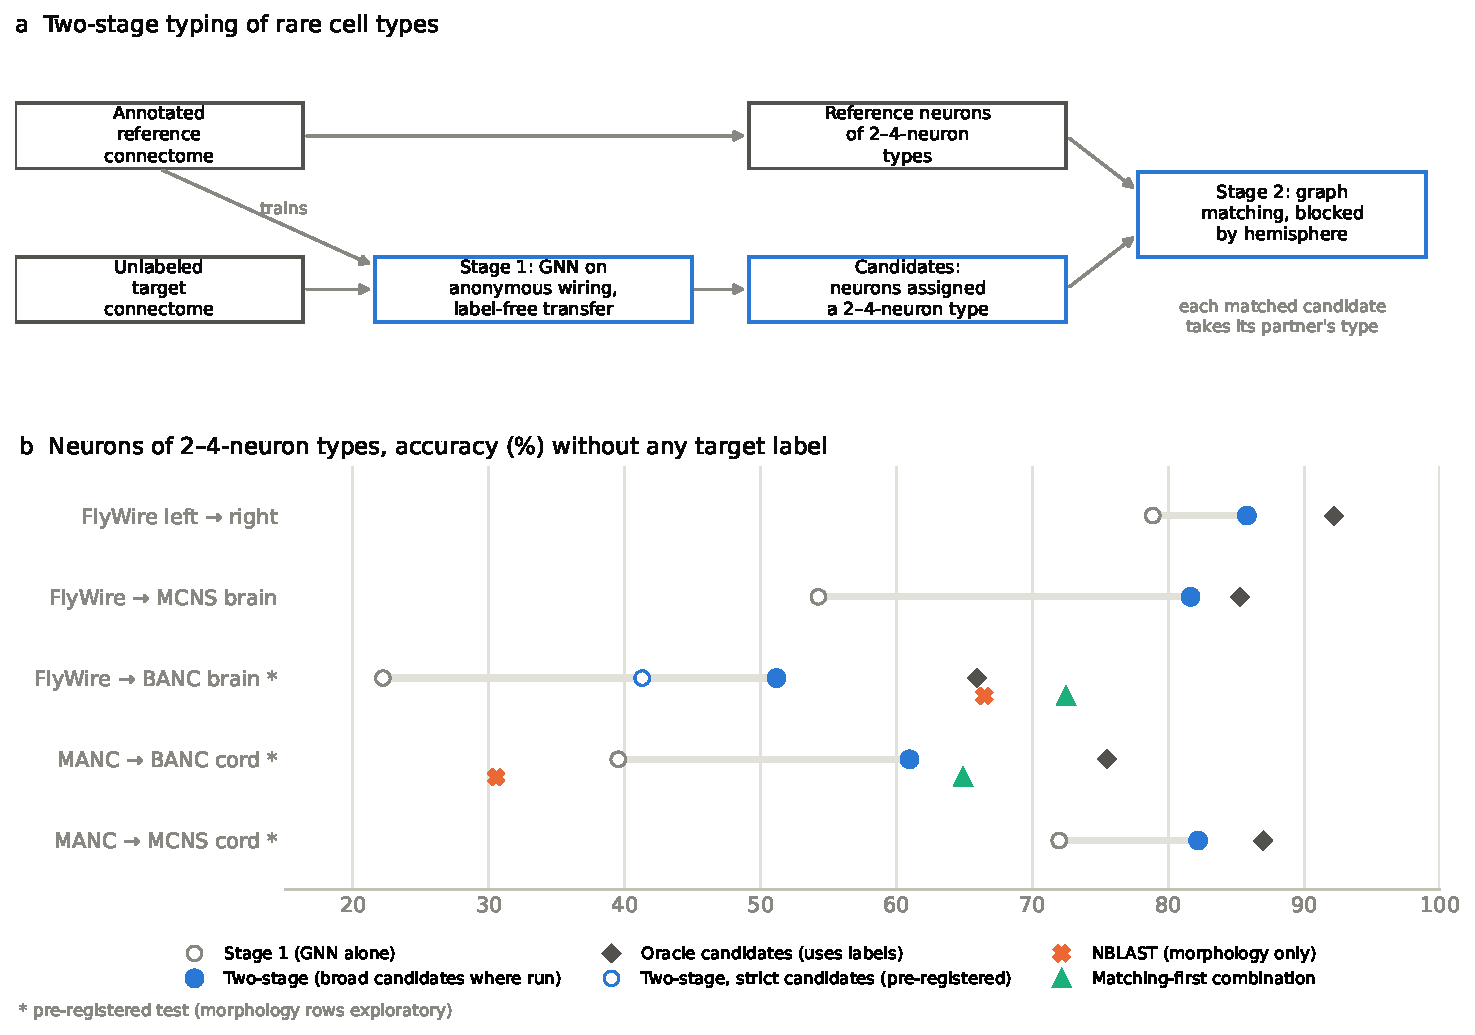
\includegraphics[width=\linewidth]{figures/rare_types.pdf}
\caption{(a) The two-stage pipeline. (b) Accuracy on target neurons of 2–4-neuron source types, without any target label, for each source → target pair: stage 1 alone, the two-stage pipeline (filled: broad candidates where run, strict within FlyWire; open: strict candidates, as pre-registered on the BANC brain), oracle candidates, and on BANC NBLAST morphology matches alone and the matching-first combination (Table~\ref{tab:names}, Section~\ref{sec:res-morph}). * pre-registered tests; the BANC-brain broad-candidate and morphology rows are exploratory.}\label{fig:1}
\end{figure}

\section{Related work}

\textbf{Cell typing from connectomes.} Fly connectomes have been annotated with thousands of types from morphology and connectivity (\citealp{scheffer2020}; \citealp{schlegel2024}; \citealp{matsliah2024}; \citealp{marin2024}). In the optic lobe, types were defined from each neuron's input and output vectors over types (\citealp{matsliah2024}). NTAC (\citealp{schwartzman2026}) automates this from labeled seeds (97.0~\% on 434 FlyWire types in our reimplementation, Supplement~\ref{sec:S-within}) and has an unsupervised mode. Learned approaches mostly use morphology (\citealp{troidl2024}) or combine it with connectivity (NeuNet; \citealp{liao2024}), where connectivity alone reached 59~\% on hemibrain classes. Across datasets, types are matched by NBLAST, connectivity alignment and combinations of both (\citealp{schlegel2024}; \citealp{bates2026}; \citealp{berg2026}). The typing methods read partner labels or are evaluated within one labeled graph; we know of no evaluation of a trained typing model transferred to an unlabeled connectome.

\textbf{Graph matching and label-free structure.} Graph matching finds the correspondence between the nodes of two graphs that best aligns their edges; the relaxed quadratic assignment problem is solved efficiently by Frank–Wolfe iterations (FAQ; \citealp{vogelstein2015}). Bisected graph matching, which also aligns the connections between hemispheres, pairs bilaterally homologous neurons of the larval connectome from connectivity alone (\citealp{pedigo2023}). Adjacency spectral embedding with Gaussian mixtures recovers neuron groups in the larval mushroom body without labels (\citealp{priebe2017}). These methods match or cluster neuron by neuron; we use graph matching as the second stage after a transferred classifier has selected the candidates, across animals and connectomes.

\textbf{Graph learning and domain adaptation.} Neurons mostly connect to neurons of other types, a heterophilic setting in which standard message passing struggles (\citealp{zhu2020}). Aggregating separately over in- and out-neighbors (Dir-GNN; \citealp{rossi2023}) raises effective homophily; our model is Dir-SAGE (\citealp{hamilton2017}; \citealp{rossi2023}) with synapse-weighted means. For transfer without target labels, prior matching is a form of label-shift correction (\citealp{saerens2002}) and of optimal transport with fixed class marginals (Sinkhorn scaling), and it mirrors reference mapping in single-cell genomics, where batch effects separate a query from an annotated atlas. Our revised selection rule uses agreement between independently trained models, which tracks their error under distribution shift (\citealp{jiang2022}).

\section{Data and methods}\label{sec:methods}

\textbf{Connectomes} (Table~\ref{tab:1}). FlyWire FAFB v783 is the source and development connectome for the brain. MCNS v1.0 (brain only) is the second development connectome; its \texttt{flywireType} annotation maps FlyWire types onto its neurons. BANC v888 and the hemibrain v1.2.1 were used only in pre-registered tests. For the nerve-cord test, MANC v1.2.1 (harmonized by the BANC project) is the source and the nerve cords of BANC and MCNS are the targets; no nerve cord was used in development. Neurons are nodes, directed edges are connections weighted by synapse count. FAFB connections have at least 5 synapses (Codex); the other connectomes are aligned to the source by fixed, label-free rules (Section~\ref{sec:align}).

\begin{table}[tbp]
\centering
\scriptsize
\caption{Connectomes. Brain columns: labels are the 434 FlyWire types with at least 20 neurons; nerve-cord columns: MANC types with at least 2 neurons (alignment reference).}\label{tab:1}
\setlength{\tabcolsep}{3pt}
\begin{tabularx}{\linewidth}{>{\raggedright\arraybackslash}p{0.14\linewidth}*{7}{>{\raggedright\arraybackslash\hspace{0pt}}X}}
\toprule
 & FAFB v783 & MCNS v1.0 brain & BANC v888 brain & Hemibrain v1.2.1 & MANC v1.2.1 & BANC v888 cord & MCNS v1.0 cord \\
\midrule
Role & source, development & development (both directions) & pre-registered tests & pre-registered test & source (cord test) & pre-registered test & pre-registered test \\
Neurons in the graph & 139,255 & 144,725 & 133,549 & 25,348 & 23,650 & 25,929 & 24,073 \\
Connections / synapses per neuron (≥ 5 synapses) & 26.8 / 364 & 35.9 / 494 & 8.6 / 100 & 26.7 / 387 & 55.1 / 969 & 16.9 / 235 & 43.4 / 759 \\
Labeled neurons (types) & 108,647 (434) & 109,901 (394) & 63,332 (409) & 7,639 (202) & 22,883 (3,901) & 22,451 (3,677) & 21,402 (3,670) \\
Particularities &  & male; synapse detection differs & sparse; types assigned by connectivity alignment to FAFB; no R1-6 photoreceptors & central brain only; 16~\% of neurons cropped & male & female; sparse & male \\
\bottomrule
\end{tabularx}
\end{table}

\textbf{Labels.} The rare-type pipeline uses all FlyWire cell types with at least 2 neurons (8,658 types, 99~\% of the labeled neurons). The \textbf{rare stratum} of a target is its labeled neurons whose type has 2–4 neurons in the source. In the nerve cord, labels are MANC cell types (3,901 types at ≥ 2, 2,452 of them with 2–4 neurons). In every target the labels are coded in the source's label space and used only for evaluation. The common-type results (Section~\ref{sec:res-common} and the Supplement) use super classes (10) and the 434 cell types with at least 20 neurons in FAFB (78~\% of neurons), the set their protocols and saved models fix; for new common-type results we recommend a minimum of 10 (779 types, 81~\%).

\textbf{Names.} Table~\ref{tab:names} defines the names of the pipeline's parts and variants, which we use throughout, together with the code options that run them.

\begin{table}[!tp]
\centering
\scriptsize
\caption{Names used in this paper. Code options refer to the scripts in \texttt{experiments/\allowbreak{}b\_\allowbreak{}gnn\_\allowbreak{}celltypes/} (see \texttt{docs/\allowbreak{}reproduce.md}).}\label{tab:names}
\begin{tabularx}{\linewidth}{>{\raggedright\arraybackslash}p{0.22\linewidth}>{\raggedright\arraybackslash}X>{\raggedright\arraybackslash}p{0.2\linewidth}}
\toprule
Name & Meaning & Code option \\
\midrule
\multicolumn{3}{l}{\emph{Pipeline}} \\
Stage 1 & The GNN trained on the source, applied to the target without labels: a selection rule chooses its preprocessing, then prior matching and NTAC refinement (Section~\ref{sec:stage1}). & \texttt{label\_\allowbreak{}free.py}, \texttt{size\_\allowbreak{}threshold.py} \\
Prior matching (coverage prior) & Rescales the GNN's class probabilities so that predicted type sizes match the source's (partial volume: the types predicted inside the covered neuropils). & \texttt{-{}-prior source} (\texttt{coverage}) \\
Stage 2; two-stage typing & Graph matching of the source's rare-type neurons to the candidates, blocked by hemisphere (Section~\ref{sec:stage2}); a matched candidate takes its partner's type, every other neuron keeps its stage-1 type. & \texttt{graph\_\allowbreak{}matching\_\allowbreak{}mcns.py} \\
\midrule
\multicolumn{3}{l}{\emph{Selection rules for stage 1's preprocessing}} \\
Type-consistency rule & The original rule: the most self-consistent labeling on the target. & \texttt{-{}-select consistency} \\
Size-and-agreement rule & The revised rule: best mean rank of type-size divergence from the prior and agreement between seeds. & \texttt{-{}-select size\_\allowbreak{}agreement} \\
\midrule
\multicolumn{3}{l}{\emph{Candidates for stage 2}} \\
Strict candidates & Neurons whose stage-1 type after NTAC is rare (the first rule). & \texttt{-{}-candidates gnn} \\
Broad candidates & Neurons whose stage-1 type before or after NTAC is rare (the improved rule). & \texttt{-{}-candidates union} \\
Morphology-augmented candidates & Broad candidates plus the neurons whose NBLAST match has a rare type. & \texttt{-{}-candidates file:\allowbreak{}nblast\_\allowbreak{}union} \\
Oracle candidates & The labeled rare-type target neurons; a diagnostic that uses labels. & \texttt{-{}-candidates oracle} \\
\midrule
\multicolumn{3}{l}{\emph{Matching options}} \\
Neck block & A third matching block for neurons that pass through the neck (nerve cord). & \texttt{-{}-passing-block} \\
Coarse fallback & Unmatched neurons typed by the ≥ 10 model; failed in the nerve cord, dropped. & \texttt{-{}-fallback} \\
\midrule
\multicolumn{3}{l}{\emph{Alignment variants of a target graph (Section~\ref{sec:align})}} \\
Unaligned / density-aligned / count-scaled & Threshold 5 / threshold matching the source's connections per neuron / counts scaled to the source's synapses per neuron. & \texttt{raw} / \texttt{density} / \texttt{scaled} (\texttt{janelia} for MCNS) \\
\midrule
\multicolumn{3}{l}{\emph{Morphology comparison (Section~\ref{sec:res-morph})}} \\
Matching-first combination & The matched type where stage 2 assigns a neuron, NBLAST's type elsewhere. & \\
NBLAST-first combination & NBLAST's type, the two-stage type where NBLAST gives none. & \\
\midrule
\multicolumn{3}{l}{\emph{Evaluation references}} \\
Alignment reference & The target's own typing, aligned to the source's types (partly by connectivity). & reference A \\
Morphology reference & BANC brain: the type of the morphology-matched FlyWire neuron (central brain). & reference B \\
Curated reference & BANC cord: BANC's curated typing. & reference B \\
\bottomrule
\end{tabularx}
\end{table}

\subsection{Stage 1: a wiring-only GNN, transferred without labels}\label{sec:stage1}

Each neuron has six features: in- and out-degree, input and output synapses, and mean synapses per input and output connection (log-scaled, z-scored). A layer computes $h'_i = W_{\mathrm{self}}\, h_i + W_{\mathrm{in}}\, \mathrm{mean}_{\mathrm{in}}(h) + W_{\mathrm{out}}\, \mathrm{mean}_{\mathrm{out}}(h)$, with means over pre- and postsynaptic partners weighted by synapse count. Cell types use 3 layers (300 epochs, class-weighted loss), super classes 4 layers (1,000 epochs); depth and options were chosen by validation macro-F1. With thousands of types the output layer and prior matching are computed in chunks, which reproduces the standard code where both can run. The model never sees a partner's label, so it applies unchanged to an unlabeled graph. Three seeds are trained throughout.

A model trained on the source is applied to the target. Every choice is made without target labels:

\begin{itemize}[leftmargin=*,itemsep=2pt]

\item \textbf{Candidate preprocessings.} Each target is built in a few alignment variants (Section~\ref{sec:align}); target features are normalized either with the source's training statistics or with the target's own; prior matching is applied with strength $\rho \in \{0, 0.25, 0.5, 0.75, 1\}$.

\item \textbf{Prior matching.} Cell-type sizes are stereotyped across flies, but a transferred classifier shifts neurons between neighboring types. We rescale its class probabilities with weights v (Sinkhorn iterations) so that the expected number of neurons per type matches the type distribution the same model predicts on its source, scaled to the target; ρ interpolates between the raw prediction and full matching ($p_k \cdot v_k^{\rho}$, renormalized).

\item \textbf{Selection.} The \emph{type-consistency rule}, used in the first test, picks the preprocessing whose labeling (mean over three seeds) is most self-consistent on the target: each neuron of a random half gets the label of its most similar neuron in the other half (synapses per partner type, weighted Jaccard), and agreement is chance-corrected (Cohen's κ). The \emph{size-and-agreement rule}, which replaced it after the first test (Section~\ref{sec:res-common}) and is used in all rare-type tests, takes the best mean rank of two other label-free properties: the Jensen-Shannon divergence of the predicted type sizes from the prior, and the agreement between the three seeds' labelings.

\item \textbf{Refinement.} NTAC on the target, seeded with the neurons on which all three seeds agree.

\end{itemize}

\subsection{Stage 2: graph matching of rare types}\label{sec:stage2}

\begin{itemize}[leftmargin=*,itemsep=2pt]

\item \textbf{Candidates} are the target neurons that stage 1 assigns to a rare type (2–4 source neurons). In the first tests these were the \emph{strict candidates}, whose type after NTAC is rare. After the BANC rare-type test, candidate selection was improved on development data (Section~\ref{sec:res-cand}); the \emph{broad candidates} take a neuron if its type before or after NTAC is rare.

\item \textbf{Matching.} Stage 2 matches the source's rare-type neurons one-to-one to the candidates. It maximizes the agreement of the two log1p(synapse) adjacency matrices among the selected neurons by Frank–Wolfe on the relaxed quadratic assignment problem (FAQ; \citealp{vogelstein2015}), from the barycenter, for 30 iterations. The assignment is block-diagonal by hemisphere and aligns both ipsilateral and contralateral connections (bisected matching; \citealp{pedigo2023}). In the nerve cord a third, pooled \emph{neck block} holds the neurons that pass through the neck (ascending and descending), whose side annotation follows the neck in MANC and the soma in the targets. Each block is padded to a square; candidates matched to padding are not assigned.

\item \textbf{Final labeling.} A matched candidate takes the type of its source neuron; every other neuron keeps its stage-1 type.

\item \textbf{Diagnostic.} With \emph{oracle candidates} (the labeled rare-type target neurons), the matching shows what perfect candidate selection would give.

\end{itemize}

At the barycenter the gradient is nearly of rank one and the exact assignment solver takes 5–10 minutes, so the first step pairs the leading singular vectors by rank. A block of about 9,300 neurons per side takes 27 minutes and 4.5 GB on a CPU, the nerve-cord blocks under 3 minutes.

\subsection{Alignment variants}\label{sec:align}

Connectomes differ in synapse detection and completeness. Each target gets variants that align one statistic with the source by a fixed rule: \emph{unaligned} (threshold 5, nothing aligned), \emph{density-aligned} (the threshold whose connections per neuron are closest to the source's) and \emph{count-scaled} (threshold 5, counts scaled so that synapses per neuron match the source's). For MCNS against FAFB we use Janelia's published scaling factor (0.581) for the last rule. In the nerve-cord test, self-connections and connections between two passing neurons, which in the targets can lie in the brain, are dropped in all three graphs.

\subsection{Pre-registration and development sandbox}\label{sec:prereg}

For each test on a new dataset, data, labels, candidates, selection rule, method, the reported numbers and explicit expectations were committed to the repository before any model was run on it: \texttt{docs/\allowbreak{}banc\_\allowbreak{}protocol.md} (BANC brain, common types), \texttt{docs/\allowbreak{}hemibrain\_\allowbreak{}protocol.md}, \texttt{docs/\allowbreak{}banc\_\allowbreak{}rare\_\allowbreak{}protocol.md} (BANC brain, rare types) and \texttt{docs/\allowbreak{}vnc\_\allowbreak{}rare\_\allowbreak{}protocol.md} (nerve cords); Table~\ref{tab:tests} summarizes them. The protocols allow only data-loading and memory fixes afterwards and require every deviation to be reported. Between tests, methods were changed only on a sandbox built from the development connectomes, with known labels: synapse counts binomially thinned before the threshold, cell types removed, the volume restricted to the central brain, or a fraction of neurons cropped (each synapse of a cropped neuron kept with probability 0.1). For partial volumes, a coverage prior uses the type distribution predicted for the FAFB neurons inside the covered volume, those with at least 10~\% of their synapses outside the optic-lobe neuropils; it needs only the list of covered neuropils.

\section{Results}

\subsection{Rare types on development data: the GNN selects, graph matching types}\label{sec:res-dev}

Having seen one or two neurons of a type on the left hemisphere, the GNN types its right-hemisphere neurons at 75.9~\% (6,438 types of 2–4 neurons, out of 8,582). These types were defined by matching neurons across hemispheres (\citealp{schlegel2024}), so the task is close to pairing homologs. We matched the left and right neurons of 2–4-neuron types by graph matching (Section~\ref{sec:stage2}) and gave each right neuron the type of its matched left neuron (Table~\ref{tab:3}). Knowing which right neurons are rare-type is an advantage the GNN does not have, so we also restricted the GNN's votes to the same candidates and made them one-to-one.

\begin{table}[tbp]
\centering
\footnotesize
\caption{The 8,142 right-hemisphere FlyWire neurons of 2–4-neuron types, typed from the left hemisphere, accuracy~\% / macro-F1.}\label{tab:3}
\begin{tabularx}{\linewidth}{>{\raggedright\arraybackslash}p{0.42\linewidth}>{\centering\arraybackslash}X>{\centering\arraybackslash}X}
\toprule
Method & Labels used on the right & Accuracy / macro-F1 \\
\midrule
GNN (mean of 3 seeds) & none & 75.9 / 0.74 \\
GNN votes, restricted to rare candidates, one-to-one & which neurons are rare-type & 79.8 / 0.81 \\
Graph matching, ipsilateral & which neurons are rare-type & 91.2 / 0.92 \\
Graph matching, bisected & which neurons are rare-type & \textbf{92.2 / 0.93} \\
GNN selects rare-type candidates, graph matching types them & none & \textbf{85.8 / 0.88} \\
\bottomrule
\end{tabularx}
\end{table}

Graph matching beats the equally restricted GNN by 12 points and wins in every region, although it sees only the edges among about 8,000 neurons per side; starting it from the GNN's votes changes nothing. The two methods combine without labels: the GNN's rare-type candidates contain 93~\% of the true rare-type neurons (84~\% precision), and matching them raises the rare types from 78.9 to 85.8~\% (GNN majority vote) and macro-F1 over all right-hemisphere neurons from 0.75 to 0.84.

Across animals the same division of labor works (Table~\ref{tab:4}). On FAFB → MCNS, stage 1 types the rare stratum at 54.2~\%, against 75.9~\% within FlyWire across hemispheres (Supplement~\ref{sec:S-transfer}). It assigns 18,479 MCNS neurons to a 2–4-neuron type; these strict candidates contain 84~\% of the labeled rare-type neurons. We matched them to the 16,365 FlyWire neurons of such types.

\begin{table}[tbp]
\centering
\footnotesize
\caption{MCNS neurons of 2–4-neuron FlyWire types (13,742 neurons, 5,370 types), without any MCNS label, accuracy~\% / macro-F1. FAFB → MCNS is the development pair; strict candidates.}\label{tab:4}
\begin{tabularx}{\linewidth}{>{\raggedright\arraybackslash}p{0.42\linewidth}>{\centering\arraybackslash}X>{\centering\arraybackslash}X}
\toprule
Method & 2–4-neuron types & All labeled MCNS neurons \\
\midrule
Stage 1 & 54.2 / 0.49 & 84.2 / 0.51 \\
Stage-1 probabilities, made one-to-one & 59.9 / 0.62 & 84.8 / 0.61 \\
Two-stage (stage 1 selects candidates, graph matching types them) & \textbf{74.5 / 0.78} & \textbf{86.3 / 0.73} \\
Same, matching started from the GNN probabilities & 74.6 / 0.78 & 86.3 / 0.74 \\
Oracle candidates & 85.3 / 0.87 & 87.4 / 0.81 \\
\bottomrule
\end{tabularx}
\end{table}

The two stages raise the rarest types by 20 points and macro-F1 over all labeled MCNS neurons from 0.51 to 0.73. The wiring does the work: matching without any GNN input is as good as matching started from the GNN's probabilities (they agree on 93~\% of candidates), while making the GNN's own probabilities one-to-one gains only 6 points. On the rare-type neurons stage 1 selects, matching reaches 89.1~\% (stage 1: 64.8~\%), and the largest gains are where the GNN is weakest (ascending, descending and other types: 25 → 66~\%; central brain: 58 → 75~\%). Graph matching between two animals is nearly as accurate as between two hemispheres (85.3~\% with oracle candidates, against 92.2~\%), so the remaining loss is mostly candidate selection. Two caveats limit this result: the stage-1 pipeline was developed on this pair, and MCNS's mapping to FlyWire types for these rare types itself comes from cross-dataset matching that uses connectivity.

\subsection{Pre-registered test on the BANC brain}\label{sec:res-banc}

We tested the two-stage pipeline on BANC under a protocol (\texttt{docs/\allowbreak{}banc\_\allowbreak{}rare\_\allowbreak{}protocol.md}, committed with the code in \texttt{0d1ee67} before either stage ran on BANC at this label set). BANC had been used before only for common types (Section~\ref{sec:res-common}). The protocol fixed stage 1's selection rule (the size-and-agreement rule, which here chose the best of the 30 candidate preprocessings), the matching (unchanged, strict candidates), two references and four expectations (Table~\ref{tab:5}). The morphology reference, the type of the FlyWire neuron matched to each BANC neuron by morphology, is independent of connectivity.

\begin{table}[tbp]
\centering
\footnotesize
\caption{Pre-registered test: BANC neurons of 2–4-neuron FlyWire types, without any BANC label, accuracy~\% / macro-F1; strict candidates. The 95~\% intervals of the alignment-reference accuracies, from resampling types, are ±1.1–1.2 points (\texttt{results/\allowbreak{}bootstrap\_\allowbreak{}ci}).}\label{tab:5}
\begin{tabularx}{\linewidth}{>{\raggedright\arraybackslash}p{0.34\linewidth}>{\centering\arraybackslash}X>{\centering\arraybackslash}X>{\centering\arraybackslash}X}
\toprule
Method & Alignment reference (14,512 neurons) & Morphology reference (13,848) & All alignment-reference neurons (88,639) \\
\midrule
Stage 1 & 22.2 / 0.19 & 21.3 / 0.18 & 47.9 / 0.19 \\
Two-stage & \textbf{41.3 / 0.47} & \textbf{40.6 / 0.47} & \textbf{51.0 / 0.40} \\
Oracle candidates & 65.9 / 0.70 & 65.5 / 0.70 & 55.0 / 0.57 \\
\bottomrule
\end{tabularx}
\end{table}

All four expectations held: the two-stage pipeline beat stage 1 by at least 10 points on both references (+19.1, 95~\% interval 18.0–20.1 from resampling types, and +19.3; +20.3 on MCNS); over all labeled neurons macro-F1 rose by at least 0.05 (0.19 → 0.40) without a loss in accuracy (+3.1 points); the rare stratum stayed below FAFB → MCNS (41.3 vs. 74.5~\%); and matching withstood BANC's sparsity better than the GNN (with oracle candidates it kept 77~\% of its MCNS accuracy, stage 1 41~\%). Unlike for common types (Section~\ref{sec:res-common}), the morphology reference gives the same result, so the gain is not an artifact of connectivity-based labels. The absolute level is limited by candidate selection: stage 1 finds only 54~\% of the rare-type neurons on BANC (84~\% on MCNS), while matching types 77~\% of those it finds correctly.

\subsection{Improving candidate selection on development data}\label{sec:res-cand}

Because BANC was then spent for rare types, we improved candidate selection on development data only. MCNS thinned to 25~\% of its synapses reproduces BANC's stage 1 (candidate recall 54.4 vs. 54.3~\%, rare-stratum accuracy 19.2 vs. 22.2~\%) and serves as a stand-in (Table~\ref{tab:6}).

\begin{table}[tbp]
\centering
\footnotesize
\caption{Candidate selection on development data: accuracy~\% / macro-F1 on the 2–4 stratum of MCNS, full and thinned to 25~\% of its synapses.}\label{tab:6}
\begin{tabularx}{\linewidth}{>{\raggedright\arraybackslash}p{0.34\linewidth}>{\centering\arraybackslash}X>{\centering\arraybackslash}X>{\centering\arraybackslash}X}
\toprule
Candidates & Recall, thinned & Thinned (25~\%) & Full MCNS \\
\midrule
Strict: stage-1 type after NTAC is 2–4 (as tested on BANC) & 54.4~\% & 47.3 / 0.53 & 74.5 / 0.78 \\
Broad: stage-1 type before or after NTAC is 2–4 & 70.0~\% & 60.1 / 0.65 & 81.6 / 0.83 \\
Oracle: labeled rare-type neurons & – & 82.0 / 0.84 & 85.3 / 0.87 \\
\bottomrule
\end{tabularx}
\end{table}

Selecting more candidates helps; ranking them better does not. The broad candidates raise recall from 54 to 70~\% on the thinned copy and from 84 to 92~\% on full MCNS, and matching stays accurate on the added neurons (81~\%). The rule has no free parameter, and a second thinning realization agrees within 1–2 points. Two further changes were tested. The coarse fallback, which types unmatched neurons with the ≥ 10 model, added 2.5–3.7 points over all labeled neurons; it was adopted and later failed in the nerve cord. Letting a FlyWire neuron match two candidates failed already here (oracle candidates: 85.3 → 76.1~\%), because candidates piled onto a few well-connected neurons.

\subsection{Pre-registered test in the nerve cords}\label{sec:res-cord}

We tested the improved pipeline in the nerve cord under a fourth protocol (\texttt{docs/\allowbreak{}vnc\_\allowbreak{}rare\_\allowbreak{}protocol.md}, committed with the code in \texttt{5119069} before any model ran on a target cord). The source is MANC, on which the GNNs were trained unchanged; the targets are the nerve cords of BANC (female, 31~\% of MANC's connections per neuron) and MCNS (a second male). The method was the one developed above (broad candidates, coarse fallback), with one disclosed change made before any model output on a cord: the neck block (Section~\ref{sec:stage2}). The alignment reference is each target's alignment to MANC, which for intrinsic neurons rests partly (BANC) or mainly (MCNS) on connectivity; the curated reference is BANC's curated typing (Table~\ref{tab:7}).

\begin{table}[tbp]
\centering
\footnotesize
\caption{Pre-registered nerve-cord test: neurons of 2–4-neuron MANC types, without any target label, accuracy~\% / macro-F1. The 95~\% intervals of these accuracies, from resampling types, are ±1.2–2.0 points (\texttt{results/\allowbreak{}bootstrap\_\allowbreak{}ci}).}\label{tab:7}
\begin{tabularx}{\linewidth}{>{\raggedright\arraybackslash}p{0.34\linewidth}>{\centering\arraybackslash}X>{\centering\arraybackslash}X>{\centering\arraybackslash}X}
\toprule
Method & BANC cord, alignment ref. (5,989) & BANC cord, curated ref. (5,257) & MCNS cord, alignment ref. (5,945) \\
\midrule
Stage 1 & 39.5 / 0.36 & 40.7 / 0.37 & 72.0 / 0.70 \\
Two-stage, strict candidates (as on the BANC brain) & 52.1 / 0.55 & 51.7 / – & 77.1 / 0.79 \\
Two-stage, broad candidates & \textbf{61.0 / 0.61} & \textbf{61.0 / 0.61} & \textbf{82.2 / 0.82} \\
Oracle candidates & 75.5 / 0.73 & 75.5 / – & 87.0 / 0.86 \\
\bottomrule
\end{tabularx}
\end{table}

Two of the four expectations held on both cords, and two did not. The broad candidates beat the strict ones by at least 3 points (+8.9 and +5.1), and the pipeline closed at least half of the gap between stage 1 and oracle candidates (0.60 and 0.68, against 0.44 for the strict-candidate pipeline on the BANC brain). The gain of at least 15 points over stage 1 held on BANC (+21.4, 95~\% interval 19.8–23.1; +20.3 against the curated reference) but not on MCNS (+10.2, 8.9–11.5), where stage 1 was already at 72.0~\% and the oracle at 87.0~\%; we had set the threshold from earlier tests and should have set it relative to the gap. The coarse fallback failed on both cords: the coarser model typed the neurons it covers worse than the fine one and cost 0.4 and 1.2 points over all labeled neurons. We therefore drop it from the recommended pipeline; the rare-type numbers do not depend on it, and without it the pipeline still gains over all labeled neurons (BANC 44.8 → 49.4~\%, MCNS 73.1 → 75.0~\%). Every neuron group gained on both cords (on BANC, descending neurons 41 → 74~\%, motor neurons 16 → 48~\%), and intrinsic neurons, whose references rest most on connectivity, gained no more than the others. Without the neck block the rare types lost 5.6–5.7 points. The cost is borne by types of 5–19 neurons (−1.5 to −2.5 points), because a fifth to a third of the candidates belong to other types and receive a rare type.

\subsection{Wiring and morphology (exploratory)}\label{sec:res-morph}

New reconstructions come with neuron shapes, and current typing starts from morphology matches (NBLAST; \citealp{costa2016}). BANC's metadata holds each neuron's NBLAST top match to FlyWire and to MANC before review. We typed each BANC neuron by its match's type and compared this with the wiring-only pipeline and with two label-free combinations (Table~\ref{tab:8}). The comparison was planned before it was run (\texttt{docs/\allowbreak{}finalize\_\allowbreak{}plan.md}, commit \texttt{9ecc769}), including the rule for how to frame its outcome. BANC's labels were known, though, so these results are exploratory. They include the first runs of broad candidates on the BANC brain.

\begin{table}[tbp]
\centering
\footnotesize
\caption{BANC neurons of 2–4-neuron source types, without any BANC label, accuracy~\% / macro-F1 (exploratory). NBLAST: the type of the top morphology match, before review. Brain: alignment reference; cord: alignment reference, with the curated reference giving the same numbers within 0.3 points.}\label{tab:8}
\begin{tabularx}{\linewidth}{>{\raggedright\arraybackslash}p{0.42\linewidth}>{\centering\arraybackslash}X>{\centering\arraybackslash}X}
\toprule
Method & BANC brain (14,512) & BANC cord (5,989) \\
\midrule
Two-stage, broad candidates (wiring only) & 51.2 / 0.57 & 61.0 / 0.61 \\
NBLAST (morphology only) & 66.5 / 0.65 & 30.5 / 0.30 \\
NBLAST-first combination & 70.7 / 0.68 & 31.3 / 0.30 \\
Two-stage, morphology-augmented candidates & 62.6 / 0.67 & 64.7 / 0.63 \\
\textbf{Matching-first combination} & \textbf{72.5 / 0.68} & \textbf{64.9 / 0.59} \\
\bottomrule
\end{tabularx}
\end{table}

On the brain, morphology alone beats wiring alone (66.5 vs. 51.2~\%), but the two err on different neurons. Where NBLAST and the pre-registered two-stage typing agree, both are right in 95~\% of cases; where they disagree, NBLAST is right in 61~\% and the matching in 16~\%. The matching-first combination, which takes the matched type where the matching assigns a FlyWire neuron and NBLAST's elsewhere, reaches 72.5~\%, 6.0 points above NBLAST alone (95~\% interval 5.1–7.1, resampling 5,416 types). The gain is the same against the morphology reference (72.0 vs. 66.8~\%), which was itself built from NBLAST matches and favors them. Every combination built on the broad-candidate matching beats NBLAST by at least 4.1 points. Morphology also helps select candidates: NBLAST's rare-type neurons raise candidate recall from 70 to 95~\%, and the matching from 51.2 to 62.6~\%, with the best macro-F1 of all rows when combined (0.71). On the cord, raw NBLAST is weak: its match has the reviewed match's type in 31~\% of cases, and its errors include neurons of another class. There the 34-point gap is to unreviewed automatic morphology, not to morphology done well. With broad candidates, the BANC brain's rare types rise from 41.3~\% (strict candidates, pre-registered) to 51.2~\%, as on the development data (Table~\ref{tab:6}). Over all labeled neurons the combination costs common types (brain 59.8 vs. 62.8~\% for the NBLAST-first combination), so the matched types should replace NBLAST's only on the rare candidates.

\subsection{Stage 1 on its own: common types}\label{sec:res-common}

The rare-type pipeline relies on stage 1 transferring without labels. We developed and tested stage 1 on common types first, the 434 FlyWire cell types with at least 20 neurons and 10 super classes; this section summarizes those results, and the Supplement gives the tables and figures.

\textbf{Within a connectome.} With labeled partners, NTAC is the best cell-type method (97.0~\%); the GNN comes close (95.3~\%, equal macro-F1) without seeing any partner label. On an unlabeled hemisphere, where the median test neuron has no synapse to a labeled partner, partner-label methods collapse on cell types (1–9~\%), while the GNN keeps 87–95~\%. The result replicates within MCNS (Supplement~\ref{sec:S-within}).

\textbf{Between complete connectomes.} Applied to MCNS, the label-free pipeline types 394 cell types at 92.6~\% after NTAC without a single MCNS label, against 96.6~\% for a GNN trained on MCNS; in the reverse direction it reaches 83.4~\% on FlyWire. The type-consistency rule ranks the 30 candidate preprocessings like their accuracy (Spearman 0.95–0.97), and prior matching corrects the type sizes (87.6~\% without, 91.2~\% with). The headline number is mostly the optic lobe: its intrinsic types, 80~\% of MCNS's labeled neurons, are typed at 97.2~\%, the other neurons at 74.0~\%. Retrained with a minimum of two neurons per type, the pipeline types MCNS at 84.2~\% over 7,064 types; this is the stage 1 of the rare-type pipeline (Supplement~\ref{sec:S-transfer}).

\textbf{Sparse and partial targets.} The first pre-registered test applied the unchanged pipeline to the BANC brain. Prior matching carried over (the best cell-type candidates use it, 13.0 and 17.5 points above the best without it), but the type-consistency rule did not: for MCNS → BANC cell types it chose a labeling that puts 77~\% of the neurons into one type (1.4~\% accuracy, against 58.0~\% for the best candidate). FAFB → BANC reached 61.7~\% after NTAC, and 32.3~\% against the morphology reference. Density explains about half of the drop (72.9~\% on a FlyWire copy thinned to BANC's density, 55.7~\% on BANC). On degraded development copies, the size-and-agreement rule had the smallest worst case and replaced the type-consistency rule; re-scored on BANC, it lands within 0.5 points of the best candidate in all four pre-registered runs, and in the later tests it chose the best candidate in four of five stage-1 runs. The hemibrain, a partial volume, cannot be typed from wiring: under the second protocol, cell types reached 19.6~\% and super classes 74.4~\%, barely above predicting the most frequent class (73.1~\%), because partners outside the volume and cut neurons remove the context the model relies on (Supplement~\ref{sec:S-sparse}).

\textbf{Value next to hand labels.} On complete targets, a few percent of hand labels propagated by NTAC type common types better: by accuracy, the GNN is worth about 1.3~\% hand labels, more for small types. No label-free signal predicts a run's accuracy reliably, but seed agreement ranks neurons: reviewing the 20~\% least-agreed neurons finds 77~\% of the errors on MCNS and 34~\% on BANC, against 20~\% for a random review (Supplement~\ref{sec:S-effort}).

\section{Discussion}

\textbf{Rare types: pairing beats classifying.} For types with two to four neurons, a trained classifier has seen one or two examples, while graph matching uses the wiring among all candidates at once. These are also the types a hand-labeling budget reaches last. Within FlyWire, where these types were defined by pairing neurons across hemispheres, matching wins by 12–16 points; between animals, the transferred GNN's role is to decide which neurons to match. That division of labor held in three pre-registered tests (across sex, at a third of the source's density, and from brain to nerve cord with a new source) and against references built from morphology or curated by hand. Candidate selection remains the bottleneck: oracle candidates are 5–25 points better than the selected ones. One-to-one matching ignores that type sizes differ between animals; a looser assignment failed, because candidates piled onto a few well-connected neurons.

\textbf{Wiring and morphology.} In practice, a new reconstruction is typed from morphology first. On BANC's brain, unreviewed NBLAST matches type rare-type neurons better than wiring alone, but the two fail on different neurons. Where they agree, the type is almost always right (95~\%), which gives a cheap confidence flag for review. Where they disagree, a neuron that graph matching assigns is better typed by the matching, which uses all of the candidates' connections at once. Morphology in turn fixes the bottleneck of the wiring pipeline: NBLAST's rare-type neurons raise candidate recall from 70 to 95~\%. We see the two-stage pipeline as a second, independent signal next to morphology, not a replacement for it. In the nerve cord, raw NBLAST matches confuse sibling types and classes, and wiring carries most of the information.

\textbf{What stage 1 contributes.} Anonymous wiring identifies cell types without labeled partners, within a connectome and across complete connectomes, which is what lets the GNN select candidates in an unlabeled target. Prior matching is its most robust ingredient: it helped on every complete or sparse target (+3.6 to +17.5 points), even with types missing from the target. None of the selection rules is reliable alone; combining a size-based and an agreement-based signal chose the best or a near-best preprocessing in every later test except the partial volume. For common types on a complete target, a few hand labels with NTAC do better, so there the GNN's niche is starting an annotation and directing review.

\textbf{What does not carry over.} Transfer degrades with reconstruction density and fails for partial volumes. Both remove context the model relies on: in a sparse reconstruction, connections; in a partial volume, partners outside it and parts of cut neurons. For typing a partial volume, a model would need to be trained on correspondingly truncated graphs or combined with morphology. Add-ons tuned on development data are fragile: the coarse fallback helped on the brain and hurt in the nerve cord. No label-free signal we tried detects an error that all seeds share, so a transferred labeling still needs a labeled spot check.

\textbf{Circularity.} Cell types were defined partly from connectivity, and cross-dataset labels (MCNS's \texttt{flywireType} and \texttt{mancType}, BANC's types, FlyWire names for hemibrain types) come from matching that uses connectivity. Agreement with them is therefore partly agreement with another connectivity-based procedure. The GNN never sees partner identities, which weakens but does not remove this concern. For rare types, the morphology reference gives the same gain as the connectivity-based one; for common types, it is the cleanest reference we found, and there FAFB → BANC reaches only 32~\%.

\textbf{On pre-registration} (Table~\ref{tab:tests}). The first two pre-registered tests contradicted part of what development data suggested, and the third confirmed it. The fourth confirmed the core method but rejected an add-on tuned on development data, and it showed that an absolute threshold can be out of reach when the baseline is already strong; thresholds relative to an oracle are the better form. Degraded copies of annotated connectomes let us diagnose and repair failures without spending a new dataset; we recommend them as a test bed for any method meant to type new reconstructions.

\begin{table}[tbp]
\centering
\footnotesize
\caption{The four pre-registered tests.}\label{tab:tests}
\begin{tabularx}{\linewidth}{>{\raggedright\arraybackslash}p{0.24\linewidth}>{\raggedright\arraybackslash}p{0.2\linewidth}>{\raggedright\arraybackslash}X>{\raggedright\arraybackslash}X}
\toprule
Test & Protocol (commit) & What was tested & Expectations \\
\midrule
BANC brain, common types & \texttt{banc\_\allowbreak{}protocol.md} (\texttt{85516a2}) & unchanged stage 1, type-consistency rule & 3: one held in every run, two only in some runs \\
Hemibrain & \texttt{hemibrain\_\allowbreak{}protocol.md} (\texttt{161cf7b}) & size-and-agreement rule, coverage prior, partial volume & 4: three held, one held for super classes only \\
BANC brain, rare types & \texttt{banc\_\allowbreak{}rare\_\allowbreak{}protocol.md} (\texttt{0d1ee67}) & two-stage pipeline, strict candidates & 4: all held \\
Nerve cords, rare types (MANC → BANC, MCNS) & \texttt{vnc\_\allowbreak{}rare\_\allowbreak{}protocol.md} (\texttt{5119069}) & broad candidates, coarse fallback, neck block & 4 per cord: two held on both, one on BANC only, the fallback failed on both \\
\bottomrule
\end{tabularx}
\end{table}

\textbf{Limitations.} The rare-type pipeline was developed on one brain pair and tested on one held-out brain and two nerve cords; every rare-type reference except BANC's morphology matches rests partly on connectivity. The morphology comparison is exploratory: it uses BANC's unreviewed NBLAST matches on a target whose labels were known, and was not repeated on MCNS; a reviewed or better-registered morphology match would be a stronger baseline. The matching uses only the edges among rare-type neurons; seeded graph matching, which would also align each candidate's connections to confidently typed common-type neurons, is the natural next step and was not tried. Single-neuron types are not predicted, and serial homologs in the nerve cord are not separated by the matching blocks. The recommended pipeline drops the fallback after the last test, so its all-neuron numbers come from runs reported in that test but not from a fresh one. The setting is transductive within a connectome. The size-and-agreement rule was chosen on 14 sandbox cases. Thinned copies cannot contain sub-threshold connections. Results depend on how neurons and classes are aligned across datasets.

\section{Conclusion}

Rare cell types, most of a fly connectome's types, can be typed without any target label by letting a transferred wiring-only GNN select the candidates and graph matching type them. The approach roughly doubles accuracy on a held-out brain (22 → 41~\%) and, with broader candidate selection, carries over to two nerve cords from a new source (40 → 61~\% and 72 → 82~\%), in pre-registered tests. It complements morphology: combined with automatic NBLAST matches, it types 73~\% of BANC's rare-type brain neurons, 6 points more than morphology alone. Candidate selection is the bottleneck, sparser reconstructions cost accuracy, and partial volumes are out of reach for wiring alone. The approach is most useful for the rare types that a labeling budget reaches last.

\section*{Code and data availability}

Code, configs, protocols and the commands for every number are in the repository (\url{https://github.com/Paradoxsmile/flybrain}; archived version: \textcolor{red}{[Zenodo DOI]}); \texttt{docs/\allowbreak{}reproduce.md} maps each table to its command and result file, and the small result summaries are committed under \texttt{results/\allowbreak{}}. Data are public (FlyWire Codex, Janelia MCNS, BANC, and the hemibrain and MANC via the BANC project's bucket). Protocols: \texttt{docs/\allowbreak{}banc\_\allowbreak{}protocol.md} (commit \texttt{85516a2}), \texttt{docs/\allowbreak{}hemibrain\_\allowbreak{}protocol.md} (\texttt{161cf7b}), \texttt{docs/\allowbreak{}banc\_\allowbreak{}rare\_\allowbreak{}protocol.md} (\texttt{0d1ee67}), \texttt{docs/\allowbreak{}vnc\_\allowbreak{}rare\_\allowbreak{}protocol.md} (\texttt{5119069}).

\bibliographystyle{plainnat}
\bibliography{references}

\clearpage
\setcounter{section}{0}
\setcounter{table}{0}
\setcounter{figure}{0}
\renewcommand{\thesection}{S\arabic{section}}
\renewcommand{\thetable}{S\arabic{table}}
\renewcommand{\thefigure}{S\arabic{figure}}
\begin{center}\Large\bfseries Supplementary material\end{center}
\suppressfloats[t]

These sections give the common-type results that Section~\ref{sec:res-common} summarizes. They use the ≥ 20 label set unless stated otherwise.

\section{Stage 1 within a connectome}\label{sec:S-within}

\textbf{Baselines}, ordered by the information they use: majority class; logistic regression on a neuron's own features; label propagation; a partner profile (logistic regression on the share of synapses per partner type, using training labels); NTAC (\citealp{schwartzman2026}; a memory-lean reimplementation checked step by step against the published package); GraphSAGE (inputs only, unweighted). Splits: random (70/15/15, stratified) and hemisphere (train and validate on one hemisphere, test on the other). Three seeds throughout (Figure~\ref{fig:S-bench}, Table~\ref{tab:S-bench}).

\begin{figure}[tbp]
\centering
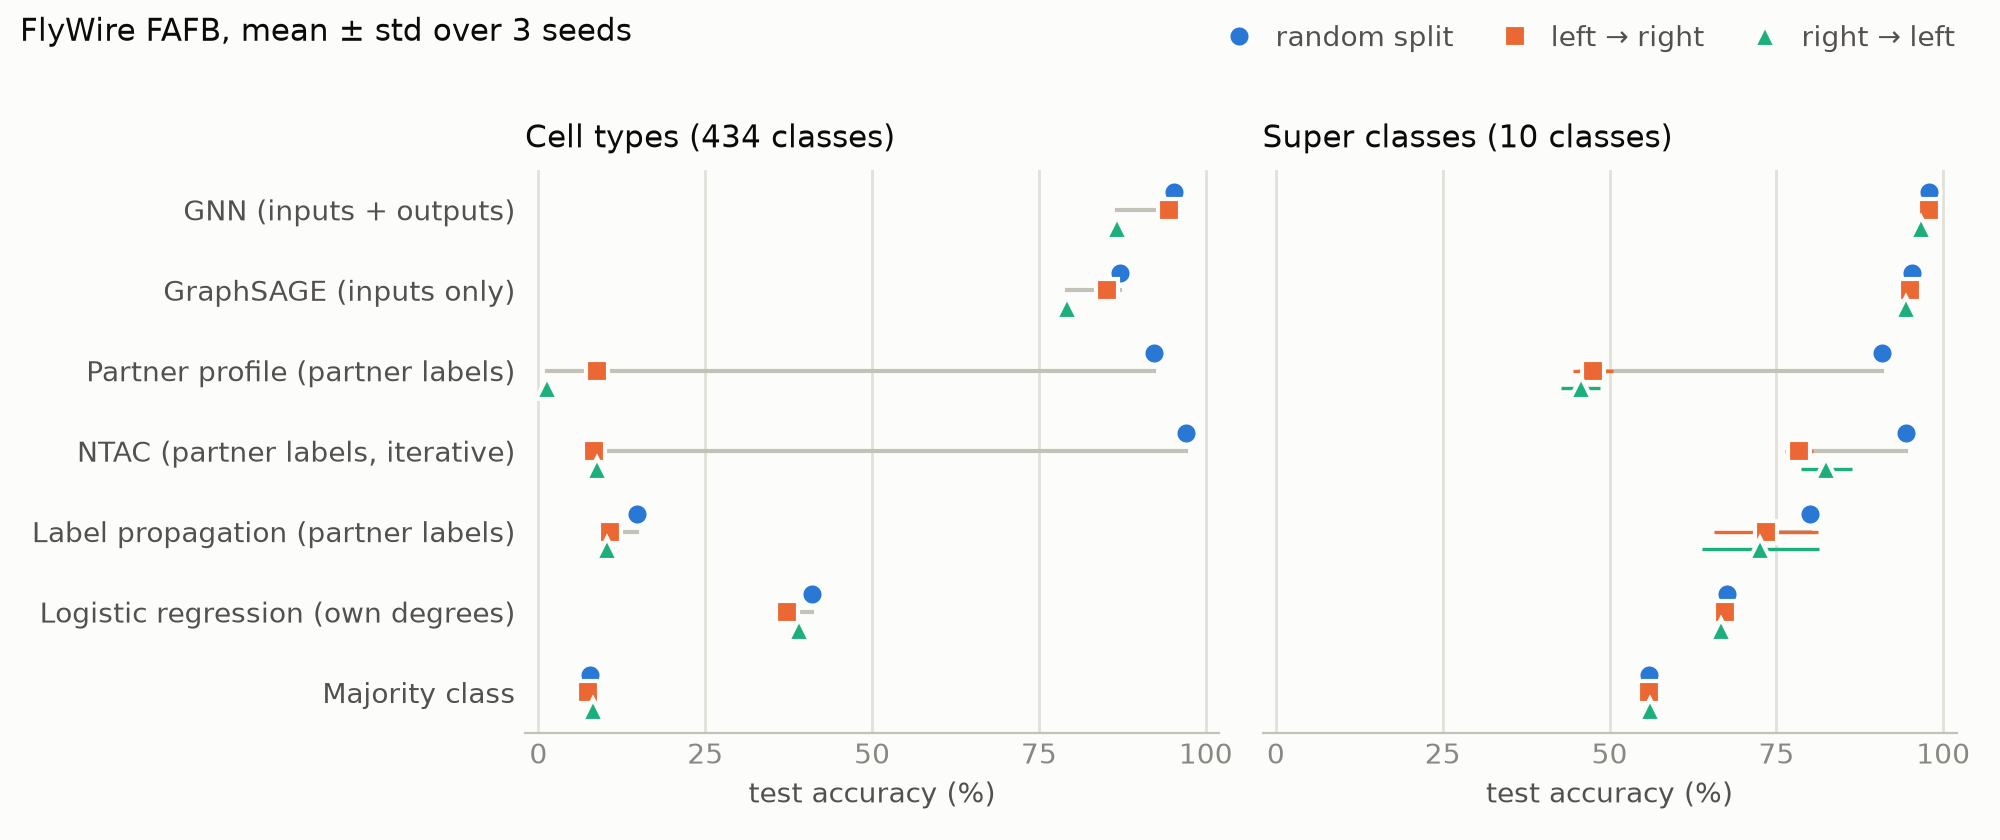
\includegraphics[width=0.92\linewidth]{../docs/benchmark_light.png}
\caption{Test accuracy on FlyWire per method and split (mean over 3 seeds, whiskers: std).}\label{fig:S-bench}
\end{figure}

\begin{table}[tbp]
\centering
\footnotesize
\caption{FlyWire, test accuracy~\% / macro-F1 (mean ± std, 3 seeds).}\label{tab:S-bench}
\begin{tabularx}{\linewidth}{>{\raggedright\arraybackslash}p{0.2\linewidth}>{\centering\arraybackslash}X>{\centering\arraybackslash}X>{\centering\arraybackslash}X>{\centering\arraybackslash}X>{\centering\arraybackslash}X>{\centering\arraybackslash}X}
\toprule
Method & Cell types, random & left → right & right → left & Super classes, random & left → right & right → left \\
\midrule
Majority class & 7.8 / 0.00 & 7.5 / 0.00 & 8.1 / 0.00 & 55.9 / 0.07 & 55.9 / 0.07 & 56.1 / 0.07 \\
Logistic regression (own degrees) & 40.9 / 0.12 & 37.3 / 0.09 & 39.0 / 0.11 & 67.6 / 0.31 & 67.2 / 0.32 & 66.7 / 0.32 \\
Label propagation & 14.7 / 0.28 & 10.7 / 0.19 & 10.3 / 0.20 & 80.1 / 0.30 & 73.4 / 0.22 & 72.6 / 0.21 \\
Partner profile (partner labels) & 92.2 / 0.79 & 8.7 / 0.10 & 1.2 / 0.10 & 90.9 / 0.60 & 47.6 / 0.28 & 45.7 / 0.23 \\
NTAC (partner labels, iterative) & \textbf{97.0 / 0.93} & 8.4 / 0.20 & 8.8 / 0.19 & 94.4 / 0.78 & 78.4 / 0.49 & 82.4 / 0.58 \\
GraphSAGE & 87.1 / 0.77 & 85.2 / 0.72 & 79.2 / 0.69 & 95.3 / 0.62 & 95.1 / 0.63 & 94.4 / 0.63 \\
GNN (Dir-SAGE, weighted) & 95.3 / \textbf{0.93} & \textbf{94.5 / 0.90} & \textbf{86.7 / 0.87} & \textbf{97.9 / 0.85} & \textbf{97.9 / 0.84} & \textbf{96.6 / 0.76} \\
\bottomrule
\end{tabularx}
\end{table}

With labeled partners, NTAC is the best cell-type method; the GNN comes close (95.3 vs. 97.0~\%, equal macro-F1) without seeing any partner label and is best on super classes. On an unlabeled hemisphere, the median test neuron has no synapse to a labeled partner (optic-lobe circuits stay on their side), and partner-label methods collapse on cell types (1–9~\%; NTAC stays below 9.4~\% at any of 40 steps), while the GNN keeps 87–95~\%. Aggregating over outputs as well as inputs adds 2–9 points over GraphSAGE of the same depth. Cell types are strongly heterophilic: only 3~\% of synapses connect neurons of the same type. The right → left gap of 8 points concentrates on photoreceptors and lamina neurons, whose outgoing synapses are underdetected in FlyWire (\citealp{matsliah2024}) and whose connection counts differ between the hemispheres.

The result replicates within MCNS: the GNN reaches 96.6~\% (random), 95.4~\% and 93.7~\% (hemispheres) on cell types, NTAC 7.8–9.5~\% on the hemispheres. Seeding NTAC with the predictions on which three GNNs agree yields 96.5 / 90.8~\% (FlyWire) and 97.1 / 96.2~\% (MCNS) on the unlabeled hemisphere.

\section{Stage 1 between complete connectomes, down to types of two neurons}\label{sec:S-transfer}

\begin{figure}[tbp]
\centering
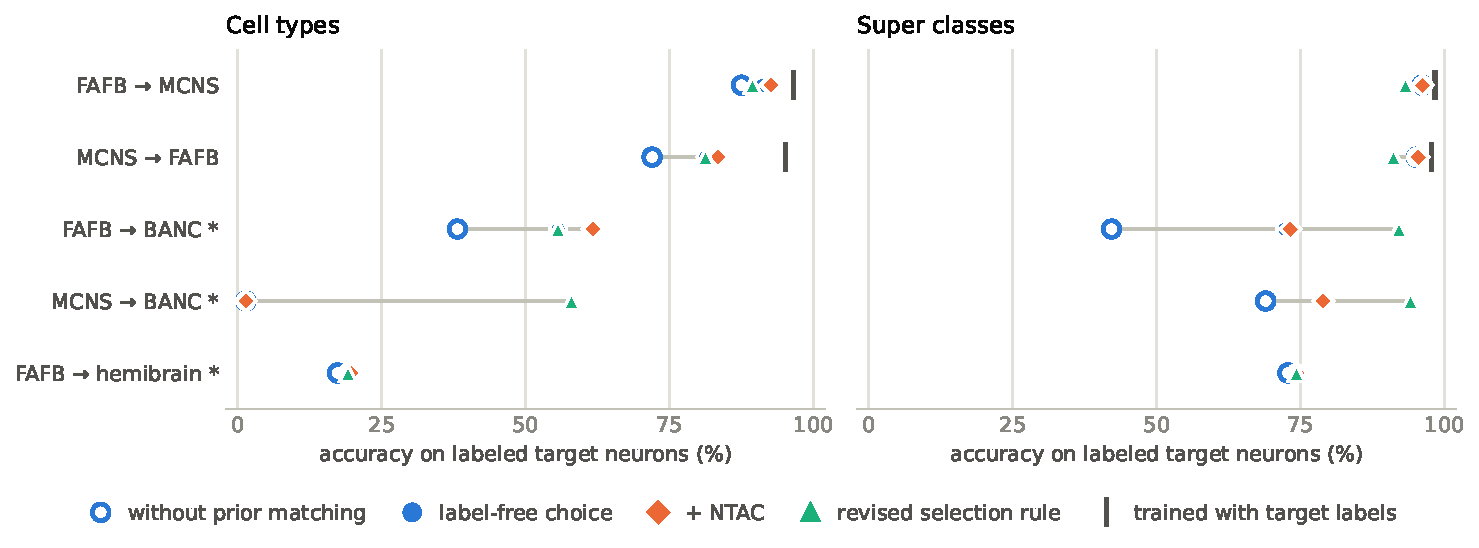
\includegraphics[width=0.92\linewidth]{figures/transfer.pdf}
\caption{Label-free transfer per scenario (accuracy on labeled target neurons). Open circles: chosen preprocessing without prior matching; filled circles: the label-free choice with prior matching; diamonds: after NTAC; triangles: the size-and-agreement rule; bars: a GNN trained with labels on the target. * pre-registered tests; their filled circles and diamonds use the rule fixed in the protocol (type consistency for BANC, size and agreement for the hemibrain).}\label{fig:S-transfer}
\end{figure}

A single FlyWire GNN applied to MCNS with a label-free normalization reaches 73–75~\% on cell types; the best alignment, found only post hoc, 85.7~\%. The label-free pipeline chooses the alignment and normalization with the type-consistency rule, which ranks the 30 candidates like their accuracy (Spearman 0.95–0.97), and prior matching corrects the type sizes: 87.6~\% without and 91.2~\% with prior matching, and \textbf{92.6~\% after NTAC, over 394 cell types without a single MCNS label}, against 96.6~\% for a GNN trained on MCNS (Figure~\ref{fig:S-transfer}). Prior matching repairs the types the transfer over- or under-fills (T5a: 2,252 → 1,714 predicted neurons for 1,664 true ones; LC21: 13 → 115 for 153). Run unchanged in the reverse direction, the pipeline reaches 83.4~\% on FlyWire (72.0~\% without prior matching; 95.2~\% trained within FlyWire). The larger gap is specific to FlyWire as a target: 2.2~\% of its neurons belong to types absent from MCNS's mapping, photoreceptors cause 21~\% of the errors (51~\% correct in the left hemisphere, 83~\% in the right), and Kenyon cell subtypes 15~\%.

\textbf{Where the accuracy comes from.} The headline number is mostly the optic lobe (Figure~\ref{fig:S-typef1}). 80~\% of MCNS's labeled neurons belong to optic-lobe intrinsic types; they are typed at 97.2~\% after NTAC and contribute 78.0 of the 92.6 points, while the other 20~\% are typed at 74.0~\%. Central-brain types transfer much worse (65.1~\%), mostly because of Kenyon cell subtypes (84~\% of their errors). The pattern repeats in the reverse direction (optic lobe 92.6~\%, all other neurons 60.9~\%) and on BANC (68.6~\% and 44.9~\%). Prior matching helps central-brain types most (+11, +16 and +26 points in the three runs).

\begin{figure}[tbp]
\centering
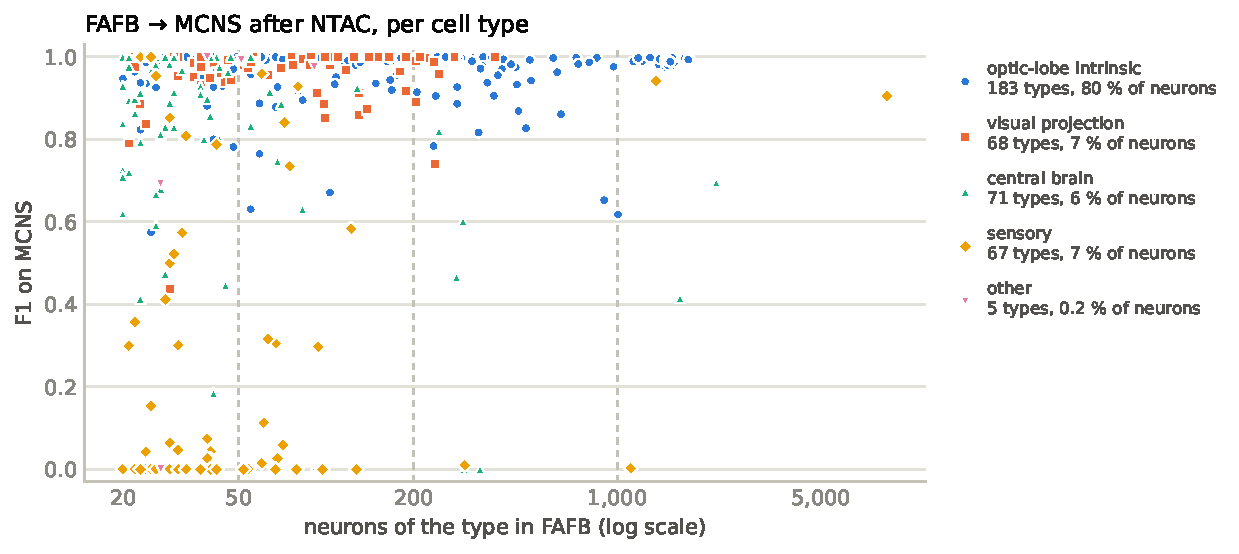
\includegraphics[width=0.92\linewidth]{figures/type_f1.pdf}
\caption{FAFB → MCNS after the label-free pipeline (+ NTAC): F1 per cell type on MCNS against the type's number of neurons in FlyWire, by region (FlyWire super class of the type). Dashed lines: the type-size bins of the stratified table.}\label{fig:S-typef1}
\end{figure}

\textbf{Smaller types.} We retrained the GNN with minimums of 10, 5, 3 and 2 neurons per type, everything else unchanged, and repeated the label-free FAFB → MCNS transfer (Table~\ref{tab:S-size}). The ≥ 2 run is stage 1 of the rare-type pipeline.

\begin{table}[tbp]
\centering
\footnotesize
\caption{Cell types by minimum type size, accuracy~\% / macro-F1 (macro-F1: mean over the true types present). FlyWire: mean ± std over 3 seeds. Transfer: label-free pipeline + NTAC.}\label{tab:S-size}
\begin{tabularx}{\linewidth}{>{\raggedright\arraybackslash}p{0.2\linewidth}>{\centering\arraybackslash}X>{\centering\arraybackslash}X>{\centering\arraybackslash}X>{\centering\arraybackslash}X>{\centering\arraybackslash}X}
\toprule
Min. size & Types (FlyWire neurons) & FlyWire, left → right & FAFB → MCNS (MCNS types) & MCNS central-brain types & Rarest bin: left → right / transfer \\
\midrule
20 & 434 (78~\%) & 94.3 ± 0.7 / 0.92 & 92.6 / 0.81 (394) & 65.1 / 0.80 (71) & 20–49: 90.7 / 77.0 \\
10 & 779 (81~\%) & 93.1 ± 1.1 / 0.87 & \textbf{93.0 / 0.80} (649) & 77.7 / 0.79 (243) & 10–19: 86.6 / 75.5 \\
5 & 2,164 (87~\%) & 89.1 ± 0.9 / 0.77 & 90.3 / 0.71 (1,694) & 72.3 / 0.70 (1,181) & 5–9: 76.4 / 71.6 \\
3 & 4,175 (93~\%) & 87.2 ± 0.8 / 0.72 & 87.6 / 0.57 (3,206) & 62.5 / 0.54 (2,542) & 3–4: see ≥ 2 \\
2 & 8,658 (99~\%) & 83.8 ± 1.1 / 0.71 & 84.2 / 0.51 (7,064) & 64.3 / 0.54 (5,371) & 2–4: 75.9 / 54.2 \\
\bottomrule
\end{tabularx}
\end{table}

Lowering the minimum from 20 to 10 costs nothing after transfer: no type-size bin is worse (20–49 neurons: 80.4 vs. 77.0~\%), and 255 types are added. Below 10, each step trades accuracy on common types for coverage: at ≥ 2 the 20–49 bin falls to 73.7~\% and the largest types (≥ 1,000 neurons) from 95.1 to 92.6~\%. With 243 central-brain types at ≥ 10, central-brain accuracy rises to 77.7~\%, and with thousands of rare ones it settles at 62–64~\%. Optic-lobe and visual projection types stay at 93–97~\% at every threshold, while small ascending, descending and other types fall to 32~\% at ≥ 2. Prior matching matters more with many types (+13.2 points at ≥ 2, +3.6 at ≥ 20). NTAC still adds 3–4 points of accuracy but lowers macro-F1 at ≥ 3 and ≥ 2 (0.62 → 0.57, 0.59 → 0.51), because it pulls neurons of rare types into common ones. Rare types transfer, but with a widening gap: types of 10–19 FlyWire neurons are typed in MCNS at 75.5~\%, of 5–9 neurons at 71.6~\% (1,045 types) and of 2–4 neurons at 54.2~\% (5,370 types, 13,742 neurons), against 86.6, 76.4 and 75.9~\% within FlyWire across hemispheres.

\section{Stage 1 on sparse and partial targets}\label{sec:S-sparse}

\textbf{BANC brain, common types.} The first pre-registered test applied the unchanged ≥ 20 pipeline to BANC (\texttt{docs/\allowbreak{}banc\_\allowbreak{}protocol.md}, \texttt{85516a2}), with the type-consistency rule (Table~\ref{tab:S-banc}).

\begin{table}[tbp]
\centering
\footnotesize
\caption{BANC, accuracy~\% / macro-F1, as pre-registered (type-consistency rule).}\label{tab:S-banc}
\begin{tabularx}{\linewidth}{>{\raggedright\arraybackslash}p{0.2\linewidth}>{\centering\arraybackslash}X>{\centering\arraybackslash}X>{\centering\arraybackslash}X>{\centering\arraybackslash}X}
\toprule
Run, label & Without prior matching & With prior matching & + NTAC & Best candidate (post hoc) \\
\midrule
FAFB → BANC, cell types & 38.2 / 0.21 & 55.7 / 0.37 & \textbf{61.7 / 0.40} & 55.7 \\
FAFB → BANC, super classes & 42.2 / 0.11 & 72.3 / 0.24 & \textbf{73.3 / 0.22} & 92.6 \\
MCNS → BANC, cell types & 1.4 / 0.00 & 1.4 / 0.00 & \textbf{1.4 / 0.00} & 58.0 \\
MCNS → BANC, super classes & 69.0 / 0.34 & 78.7 / 0.33 & \textbf{79.0 / 0.31} & 94.3 \\
\bottomrule
\end{tabularx}
\end{table}

Of three pre-registered expectations, the first (selected candidate within 2 points of the best) held in one of four runs; the second (the pipeline beats every candidate without prior matching on cell types) held for FAFB → BANC only; the third (cell-type accuracy below FAFB → MCNS) held. Prior matching carried over: the best cell-type candidates use full prior matching, 13.0 and 17.5 points above the best candidates without it, although BANC lacks the R1-6 photoreceptors that the prior expects (prior matching fills R1-6 with 10,800 neurons, 20~\% of the remaining errors). The selection did not: for MCNS → BANC cell types it chose a labeling that puts 77~\% of the neurons into one type; such a labeling is self-consistent on the graph, and the chance correction does not penalize the collapse enough. Against the morphology reference (central brain only), FAFB → BANC reaches 32.3~\% after NTAC; the optic lobe reaches 67.4~\% against BANC's own types.

\textbf{Density.} BANC's brain graph is sparse: the median neuron has 30 input synapses from other neurons in the graph and 4 input partners (FlyWire: 152 and 14). Thinned copies of FlyWire, which keep each synapse with probability p before the threshold of 5, reproduce BANC's statistics at p ≈ 0.35–0.4. Transfer between independently thinned copies isolates density from all other differences (Figure~\ref{fig:S-thin}).

\begin{figure}[tbp]
\centering
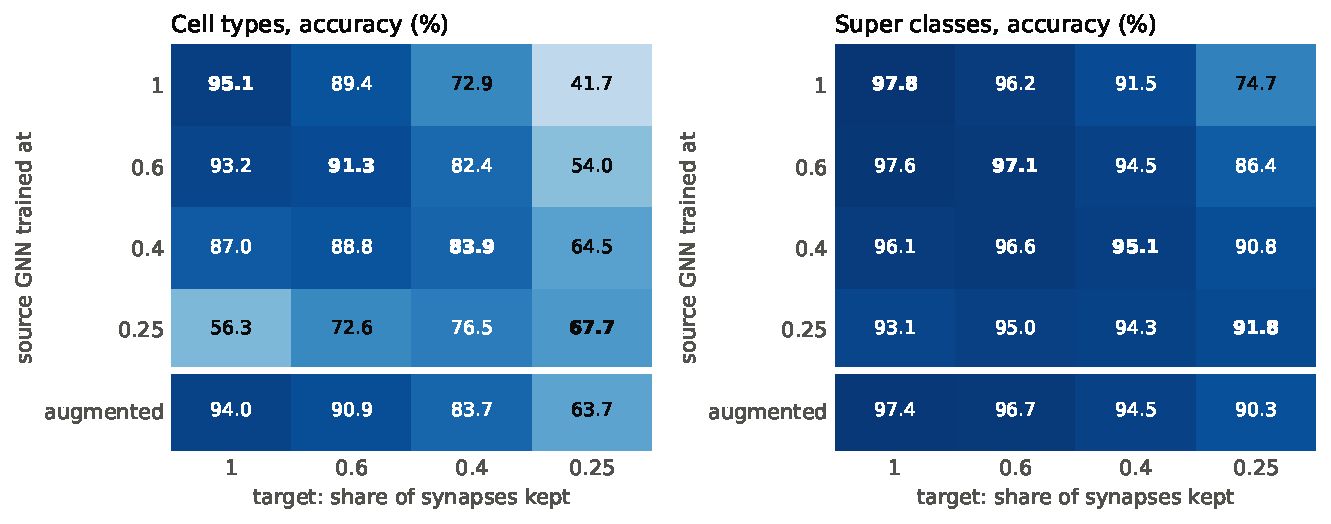
\includegraphics[width=0.92\linewidth]{figures/thinning.pdf}
\caption{Transfer between thinned FlyWire copies, with prior matching (test split, mean over 3 seeds). Rows: density of the source copy the GNN was trained on; ``augmented'': one GNN trained with a random density in [0.25, 1] per epoch.}\label{fig:S-thin}
\end{figure}

\begin{itemize}[leftmargin=*,itemsep=2pt]

\item \textbf{Density explains about half of the drop on BANC}: the full-density GNN reaches 72.9~\% on a copy at BANC's density, against 55.7~\% on BANC.

\item \textbf{A sparser target is best served by a source of its density} (83.9 vs. 72.9~\% at p = 0.4), but accuracy falls even then (95.1 → 67.7~\% on the diagonal): a sparse reconstruction loses information.

\item \textbf{A denser target is benign with prior matching}: a GNN trained at p = 0.4 reaches 87.0~\% on the full-density copy (70.0~\% without prior matching).

\item \textbf{One GNN trained with random thinning approaches the density-matched GNNs on every target} (94.0, 90.9, 83.7, 63.7~\% against 95.1, 91.3, 83.9, 67.7~\%), without knowing the target's density.

\item On BANC itself, neither density-matched nor augmented GNNs beat the full-density GNN (51.2 and 55.0 vs. 55.7~\%, exploratory). There, the density-aligned variant, which lowers the threshold to 2 synapses, recovers strong connections that survive as weak ones; the thinned copies cannot show this, because FlyWire's public connections start at 5 synapses.

\end{itemize}

\textbf{Selection.} Degraded copies of the development connectomes with known labels (FAFB → MCNS at 100, 50 and 20~\% of MCNS's synapses, MCNS → FAFB at 100 and 35~\%, FAFB → MCNS without R1-6, with and without bounded prior matching) reproduce the BANC failure: at 20~\% density, type consistency ranks the candidates inversely to their accuracy (Spearman −0.68 for cell types). Table~\ref{tab:S-rules} compares label-free selection rules.

\begin{table}[tbp]
\centering
\footnotesize
\caption{Gap between the chosen and the best candidate preprocessing, points, mean / worst.}\label{tab:S-rules}
\begin{tabularx}{\linewidth}{>{\raggedright\arraybackslash}p{0.42\linewidth}>{\centering\arraybackslash}X>{\centering\arraybackslash}X}
\toprule
Rule & Sandbox (14 cases) & BANC re-scored (6 cases, exploratory) \\
\midrule
Type consistency (original) & 4.1 / 26.7 & 19.9 / 56.6 \\
Type sizes closest to the prior & 4.1 / 26.0 & 0.6 / 1.8 \\
Consistency + seed agreement, collapse guard & 1.1 / 8.9 & 1.5 / 5.8 \\
\textbf{Type sizes + seed agreement (size-and-agreement rule)} & \textbf{1.3 / 4.0} & \textbf{1.1 / 6.3} \\
\bottomrule
\end{tabularx}
\par\smallskip\raggedright\footnotesize Cases are runs × labels. BANC: the four pre-registered runs (FAFB → BANC and MCNS → BANC, cell types and super classes) and, exploratory, FAFB → BANC with GNNs trained on FlyWire thinned to p = 0.4 (both labels). The worst case of the size-and-agreement rule (6.3) is the density-matched super-class run.
\end{table}

Type consistency is the best single signal on complete graphs and fails on sparse ones; the type-size divergence behaves the other way round; seed agreement tracks accuracy closely on complete graphs (Spearman 0.98 for MCNS → FAFB cell types). The size-and-agreement rule had the smallest worst case on the sandbox and was chosen there, before it was computed on BANC. Re-scored on BANC (the candidates' accuracies were known from the pre-registered runs), it lands within 0.5 points of the best candidate in all four pre-registered runs, including the collapsed one (58.0 instead of 1.4~\%). In the two pre-registered rare-type tests on new targets it chose the best candidate in four of five stage-1 runs and missed by 1.9 points in the fifth. Two candidate fixes did not help: bounding prior matching to avoid filling missing types (fewer wrong R1-6, but lower accuracy), and estimating target type sizes by EM (\citealp{saerens2002}), which amplified the classifier's errors.

\textbf{Partial volumes.} The hemibrain covers the central brain without the optic lobes; 77~\% of FlyWire's labeled neurons belong to types it does not contain. This breaks the shared assumption of prior matching, the size-based selection and normalization by the target's own statistics: that the target has the source's composition. In the sandbox (MCNS restricted to the central brain, 16~\% cropped), the best candidate for the same central-brain neurons fell from 69.9~\% (full volume) to 46.9~\% (partial) and 36.3~\% (partial and cropped); the coverage prior raised it from 30.5 to 36.3~\% and was adopted. The second pre-registered test (\texttt{docs/\allowbreak{}hemibrain\_\allowbreak{}protocol.md}, \texttt{161cf7b}) was also the first test of the size-and-agreement rule. The harmonized hemibrain edgelist repeats rows (931,329 exact copies), which we drop; within its volume the hemibrain then has FlyWire's density (Table~\ref{tab:S-hemi}).

\begin{table}[tbp]
\centering
\footnotesize
\caption{Hemibrain, accuracy~\% / macro-F1, as pre-registered (size-and-agreement rule, coverage prior).}\label{tab:S-hemi}
\begin{tabularx}{\linewidth}{>{\raggedright\arraybackslash}p{0.2\linewidth}>{\centering\arraybackslash}X>{\centering\arraybackslash}X>{\centering\arraybackslash}X>{\centering\arraybackslash}X>{\centering\arraybackslash}X}
\toprule
Label & Without prior matching & With prior matching & + NTAC & Best candidate (post hoc) & Type-consistency rule \\
\midrule
Cell types & 17.3 / 0.09 & 19.1 / 0.09 & \textbf{19.6 / 0.09} & 25.5 & 7.8 \\
Super classes & 72.8 / 0.20 & 74.3 / 0.20 & \textbf{74.4 / 0.19} & 78.4 & 72.8 \\
\bottomrule
\end{tabularx}
\end{table}

Of four expectations, the selection was within 5 points of the best candidate for super classes (4.1) but not for cell types (6.4); the coverage prior gave a better best candidate than the FlyWire prior, by little for cell types (25.5 vs. 24.9~\%) and decisively after selection for super classes (74.4 vs. 34.5~\%); complete neurons were typed better than cropped ones (22.8 vs. 12.2~\% on cell types); and cell-type accuracy stayed below 60~\%. Super-class accuracy is barely above predicting the most frequent class (73.1~\%); visual projection neurons, whose dendrites lie in the missing optic lobe, are typed correctly in 5~\% of cases, central-brain neurons in 28~\%. Partners outside the volume and cut neurons remove the context the model relies on.

\section{Stage 1 next to hand labels, and estimating accuracy without labels}\label{sec:S-effort}

A team typing a new connectome would not rely on wiring alone; it can label neurons by hand and propagate the labels with NTAC. On the ≥ 20 label set, we labeled k~\% of each type's neurons at random (three draws) and compared NTAC seeded with the hand labels only, NTAC seeded with the hand labels plus the GNN predictions on which three seeds agree (fixed seeds, as in Supplement~\ref{sec:S-within}), and NTAC with the label-free pipeline as a fallback for types that have no hand label (Figure~\ref{fig:S-effort}, Table~\ref{tab:S-effort}).

\begin{figure}[tbp]
\centering
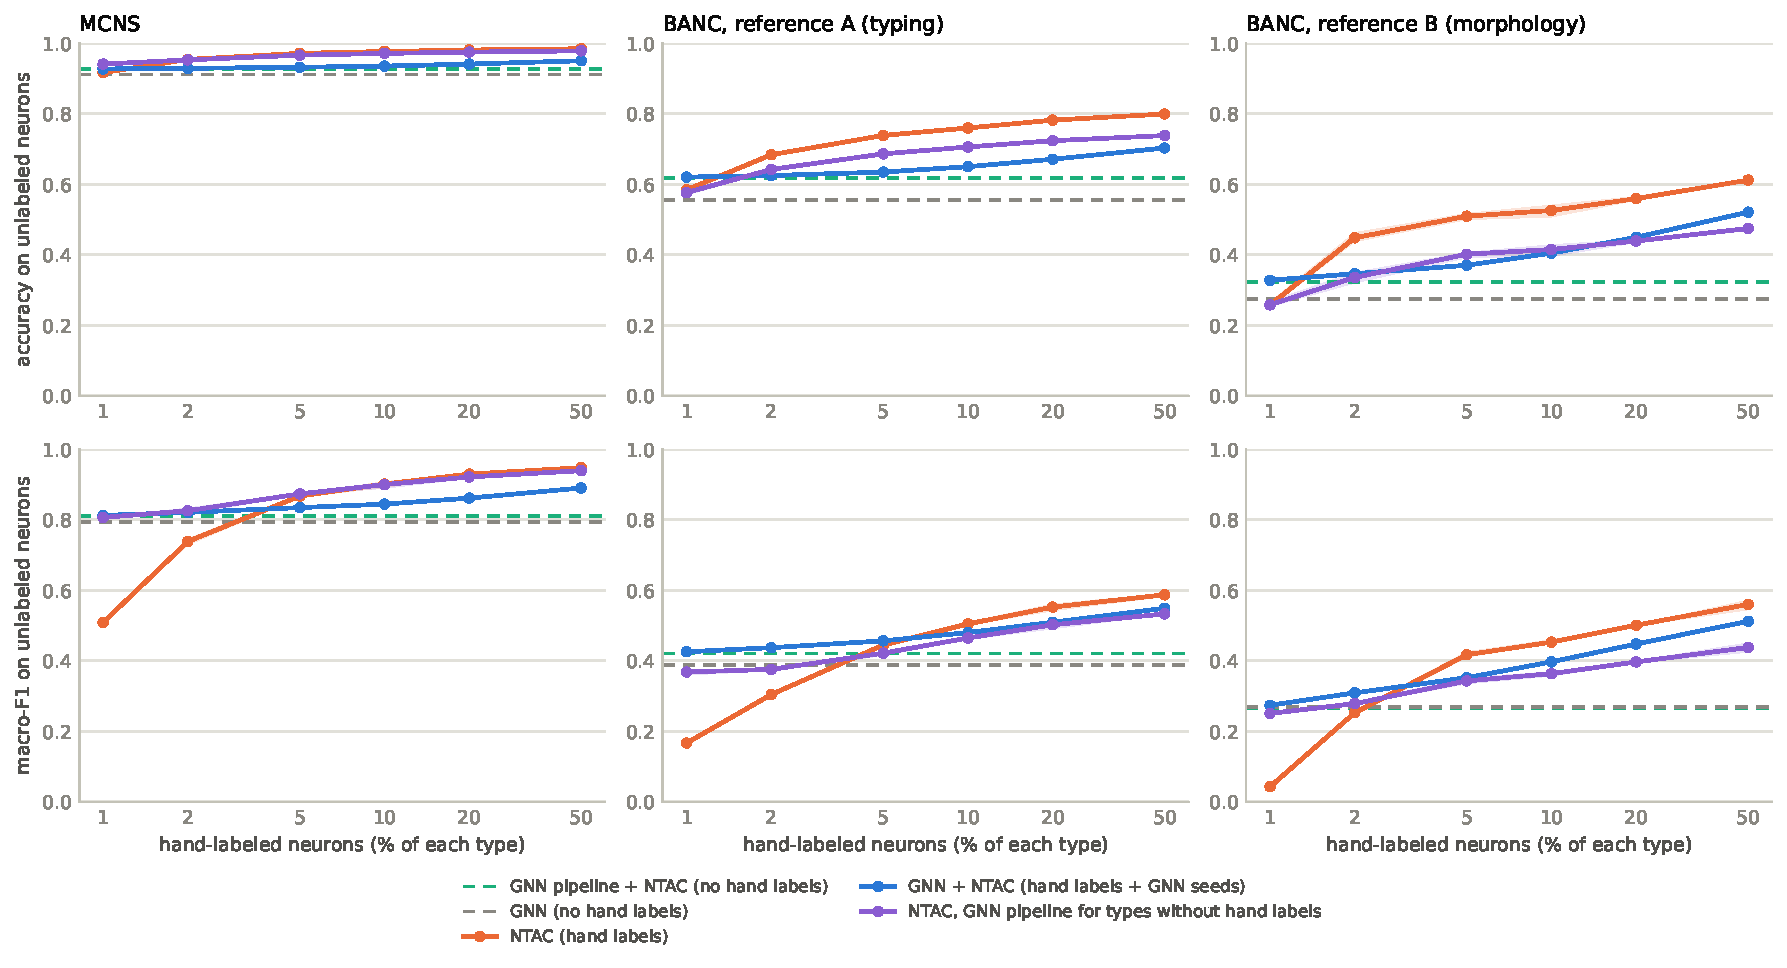
\includegraphics[width=0.92\linewidth]{figures/label_effort.pdf}
\caption{Accuracy and macro-F1 on the neurons without a hand label, against the share of each type labeled by hand (mean over three draws, ≥ 20 label set). Dashed: the label-free pipeline without hand labels.}\label{fig:S-effort}
\end{figure}

\begin{table}[tbp]
\centering
\footnotesize
\caption{Hand labels NTAC alone needs (\% of each type) to match GNN-seeded NTAC at k = 1~\%.}\label{tab:S-effort}
\begin{tabularx}{\linewidth}{>{\raggedright\arraybackslash}p{0.34\linewidth}>{\centering\arraybackslash}X>{\centering\arraybackslash}X>{\centering\arraybackslash}X}
\toprule
Target & GNN + NTAC at 1~\% & NTAC alone, by accuracy & NTAC alone, by macro-F1 \\
\midrule
MCNS & 92.7 / 0.81 & 1.2~\% & 3.4~\% \\
BANC, BANC's types & 62.1 / 0.43 & 1.3~\% & 4.4~\% \\
BANC, morphology reference & 32.8 / 0.27 & 1.3~\% & 2.3~\% \\
\bottomrule
\end{tabularx}
\end{table}

By accuracy, the GNN is worth about 1.3~\% hand labels on all three references; from 2~\% on, NTAC alone is better (MCNS at 5~\%: 97.2 vs. 93.2~\%; BANC: 73.9 vs. 63.5~\%). The GNN's contribution is larger for small types: random labeling at 1~\% leaves types with fewer than 50 neurons unlabeled, which NTAC cannot assign, and GNN-seeded NTAC matches the macro-F1 that NTAC alone reaches only with 2.3–4.4 times as many hand labels. Fixed GNN seeds are the wrong way to combine both once hand labels exist, because NTAC never revises them: in the MCNS central brain, GNN-seeded NTAC gains 9 points between 1 and 50~\% hand labels, NTAC alone 27 points. The fallback variant is best at 1~\% on MCNS (94.1~\%, macro-F1 0.81) but hurts on BANC, where the transferred labels are less reliable. The rare-type pipeline was not part of this comparison.

\textbf{Can one tell without labels how good a labeling is?} We fitted simple linear predictors of accuracy from the label-free properties of all 1,200 candidate labelings of the development runs and the sandbox, and tested them on BANC and the hemibrain. The pre-specified predictor (seed agreement and type-size divergence) missed by 12.8 points on average (median 8.4). It was accurate on complete targets with a non-collapsed labeling (FAFB → BANC cell types: 0.5 points). It failed when all seeds made the same error: on the collapsed MCNS → BANC labeling (predicted 44.5~\%, true 1.4~\%) and on hemibrain super classes with the FlyWire prior (seed agreement 0.94, 34.7~\% correct). Seed agreement does rank neurons and types where the transfer works: reviewing the 20~\% least-agreed neurons finds 77~\% of the errors on MCNS, 55~\% on FlyWire and 34~\% on BANC (random review: 20~\%), and per type it correlates with F1 (Spearman 0.54–0.66). On the hemibrain, where 80~\% of the labels are wrong, it is no better than random.

\end{document}
